\documentclass[12pt,a4paper]{article}

\usepackage[utf8]{inputenc}
\usepackage[ngerman]{babel}
\usepackage[T1]{fontenc}
\usepackage{amsmath}
\usepackage{amsfonts}
\usepackage{amssymb}
\usepackage{graphicx}
\usepackage[left=2cm,right=2cm,top=2cm,bottom=2cm]{geometry}
\usepackage{multicol}
\usepackage{booktabs}
\usepackage[hidelinks]{hyperref}
\usepackage{tikz}
\usepackage{pgfplots}
\usepackage{blindtext}
\usepackage{array}
\usepackage{multirow}
\usepackage{bigdelim}
\usepackage{colortbl}
\usepackage{fancyhdr} 
\usepackage{tabularx}
\usepackage{xcolor}
\usepackage{color}
\usetikzlibrary{decorations.text}
\usetikzlibrary{tikzmark}
\pagestyle{fancy} 
	\fancyhf{} 
	\fancyhead[L]{
\includegraphics[scale=0.05]{Bilder/dhbw.png}} 
	\fancyhead[C]{\slshape Netztechnik} 
	\fancyhead[R]{\slshape LaTeX Version}
	\fancyfoot[C]{\thepage}
\usepackage{helvet}
\renewcommand{\familydefault}{\sfdefault}

\title{Netztechnik}
\author{\slshape Robin Rausch, Florian Maslowski}
\date{\slshape \today}

\begin{document}
	\pagenumbering{Roman}
	\maketitle
	\tableofcontents
	\newpage
	\pagenumbering{arabic}
	\section{Grundlagen}
		\subsection{OSI-7-Schichten-Modell}
			\textbf{Merkhilfe:} Please Do Not Throw Salami Pizza Away.\\
			Zweck des Open-System-Interconnection-Modells ist, Kommunikation über unterschiedlichste technische Systeme hinweg zu beschreiben und die Weiterentwicklung zu begünstigen.\newline\newline
			\begin{minipage}{.5\textwidth}
				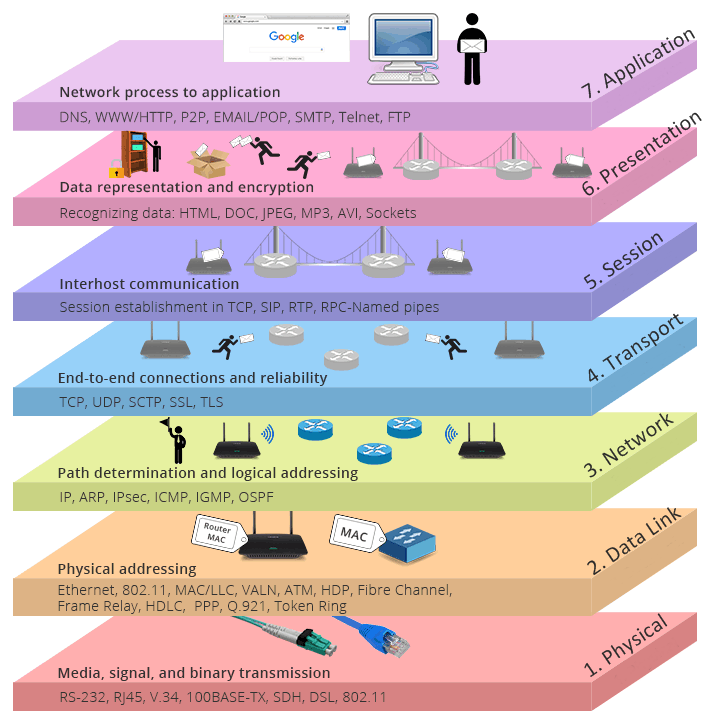
\includegraphics[scale=.45]{Bilder/OSI-Modell1} %aus Abi-Lernzettel kopiert
			\end{minipage}
			\begin{minipage}{.5\textwidth}
				\textbf{Hauptaufgaben der Schichten:}
				\begin{itemize}
					\item Schicht 7: Anwendungen für Benutzer
					\item Schicht 6: Darstellung der Daten in verständliche Formate (jpg, ASCII)
					\item Schicht 5: Steuerung der Verbindung
					\item Schicht 4: Zuordnung der Datenpakete zu den Ports
					\item Schicht 3: Vermittelt Datenpakete
					\item Schicht 2: Fehlerfreie Übertragung
					\item Schicht 1: Bit-Übertragung 
				\end{itemize}
			\end{minipage}
			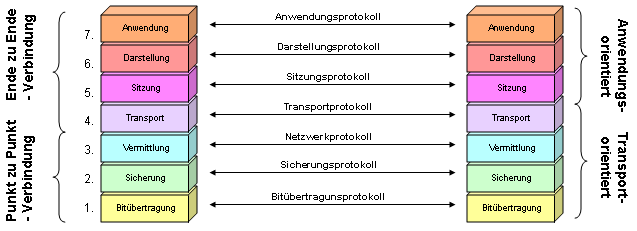
\includegraphics[scale=.75]{Bilder/OSI-Modell2} %aus Abi-Lernzettel kopiert

		\subsection{Protokolle (+Zuordnung)}
			\subsubsection{Layer 1: Physical Layer - Bitübertragungsschicht}
				Diese Schicht beschreibt die physische Übertragung der Daten. Zusammenfassend geht es hierbei hauptsächlich um Kabel und Sender/Empfänger. \textcolor{red}{??}

			\subsubsection{Layer 2: Data Link Layer - Sicherungsschicht}
				Hier wird der Ethernet Frame zusammengebaut und NIC und MAC-Adressen verwendet. Die MAC-Adresse fällt deshalb auch unter die Schicht 2 und wird später genauer erklärt. \textcolor{red}{??}

			\subsubsection{Layer 3: Network-Layer - Vermittlungsschicht}
				In der 3. Schicht werden Verbindungen zu Hostsystemen (auch außerhalb des Netzes) aufgebaut. Darunter fallen beispielsweise Router.

			\subsubsection{Layer 4: Transport Layer - Transportschicht}
				Layer 4 stellt eine transparente Datenübertragung zwischen Endsystemen zur Verfügung. Darunter fallen beispielsweise TCP und UDP:\newline\newline
				Bei TCP wird vor dem Datentransport eine Verbindung zwischen den Parteien aufgebaut und während des gesamten Datenaustausches gehalten. Nach Abschluss des Datenflusses wird die Verbindung wieder abgebaut. Verwendet werden hierbei Timer, Wiederholungen, Flusskontrolle, Windowing/Stop and Wait und Multiplexing um eine Verbindung mehrfach nutzen zu können.\newline\newline
				Bei UDP werden die Daten in das Netzwerk in Richtung Empfänger gesendet, ohne dass der Sender weiß, ob der Empfänger empfangsbereit ist. Damit sind die oben aufgeführten Mechanismen, wie Flusskontrolle und Wiederholungen in den überlagerten Schichten zu bearbeiten.

			\subsubsection{Layer 5: Session Layer - Sitzungsschicht}
				Diese Schicht ist die erste anwendungsorientierte Schicht und behandelt Sitzungsabläufe und Synchronisationspunkte. Wenn ein Fehler auftritt, kann auf diese Synchronisationspunkte aufgesetzt werden. Ebenso fallen die Betriebsarten(Simplex, Half-Duplex und Full-Duplex) und Phasen(Verbindungsaufbau, Datenübertragung und Verbindungsaufbau) unter diese Schicht. \textcolor{red}{??}

			\subsubsection{Layer 6: Presentation Layer - Darstellungsschicht}
				Unterschiedliche Rechner haben aufgrund unterschiedlicher Betriebssysteme unterschiedliche Darstellungsformen der Daten. Soll eine Applikation auf unterschiedlichen Betriebssystemen ablaufen können, sind Konvertierungen durchzuführen.
				Hier werden folgende Umsetzungen abgewickelt:\newline
				Zeichensätze (ASCII, EBCDIC), Interpretation von Bytes MSB (Most Significant Bit)/LSB (Least Significant Bit), Kompression/Dekompression und Verschlüsselung/Entschlüsselung

			\subsubsection{Layer 7: Application Layer - Anwendungsschicht}
			Diese Schicht bildet die Schnittstelle zum Anwender (User). Beispiel hierfür sind:\newline
			FTP File Transfer Protocol, SMTP Simple Mail Transfer Protocol, SNMP Simple Network Management Protocol und DNS Domain Name Service

	\section{MAC-Adresse}
	Um Informationen im Ether / Internet zuverlässig und zielgenau verschicken zu können, muss jedes Endgerät im Netz seine eigene individuelle Kennung besitzen!\newline $\longrightarrow$ \emph{MAC Adresse}\newline Die MAC Adresse ist in den ROM der Network Interface Card eines jeden Gerätes eingebrannt. Die MAC ist also keine virtuelle Softwarekennung, sondern eine durchaus physisch mit dem Gerät verbundene Kennnummer. Die MAC-Adresse gehört zur OSI Schicht 2 und besteht aus 48bit welche in 4 Teile eingeteilt werden:
	\begin{center}
		\begin{figure}
			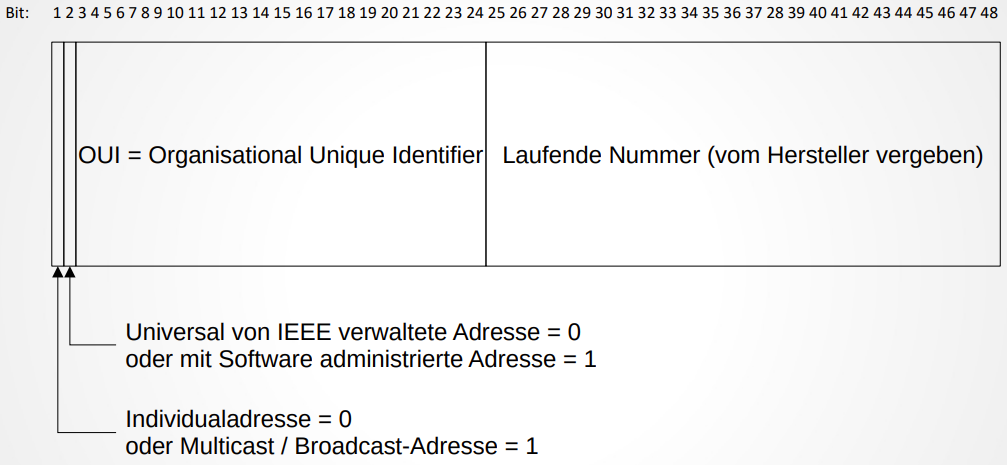
\includegraphics[width=\textwidth]{Bilder/MAC-Adresse.PNG}
		\end{figure}
	\end{center}
	\begin{center}
		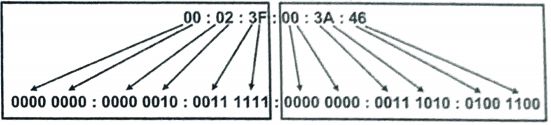
\includegraphics[scale=1]{Bilder/MAC.png}
		\begin{tabularx}{14cm}{XX}
			3 Byte OUI (Herstellerkennung)&3Byte Gerät-Seriennummer
		\end{tabularx}
	\end{center}

	\section{Kabel}
		\subsection{Verkehrsarten}
			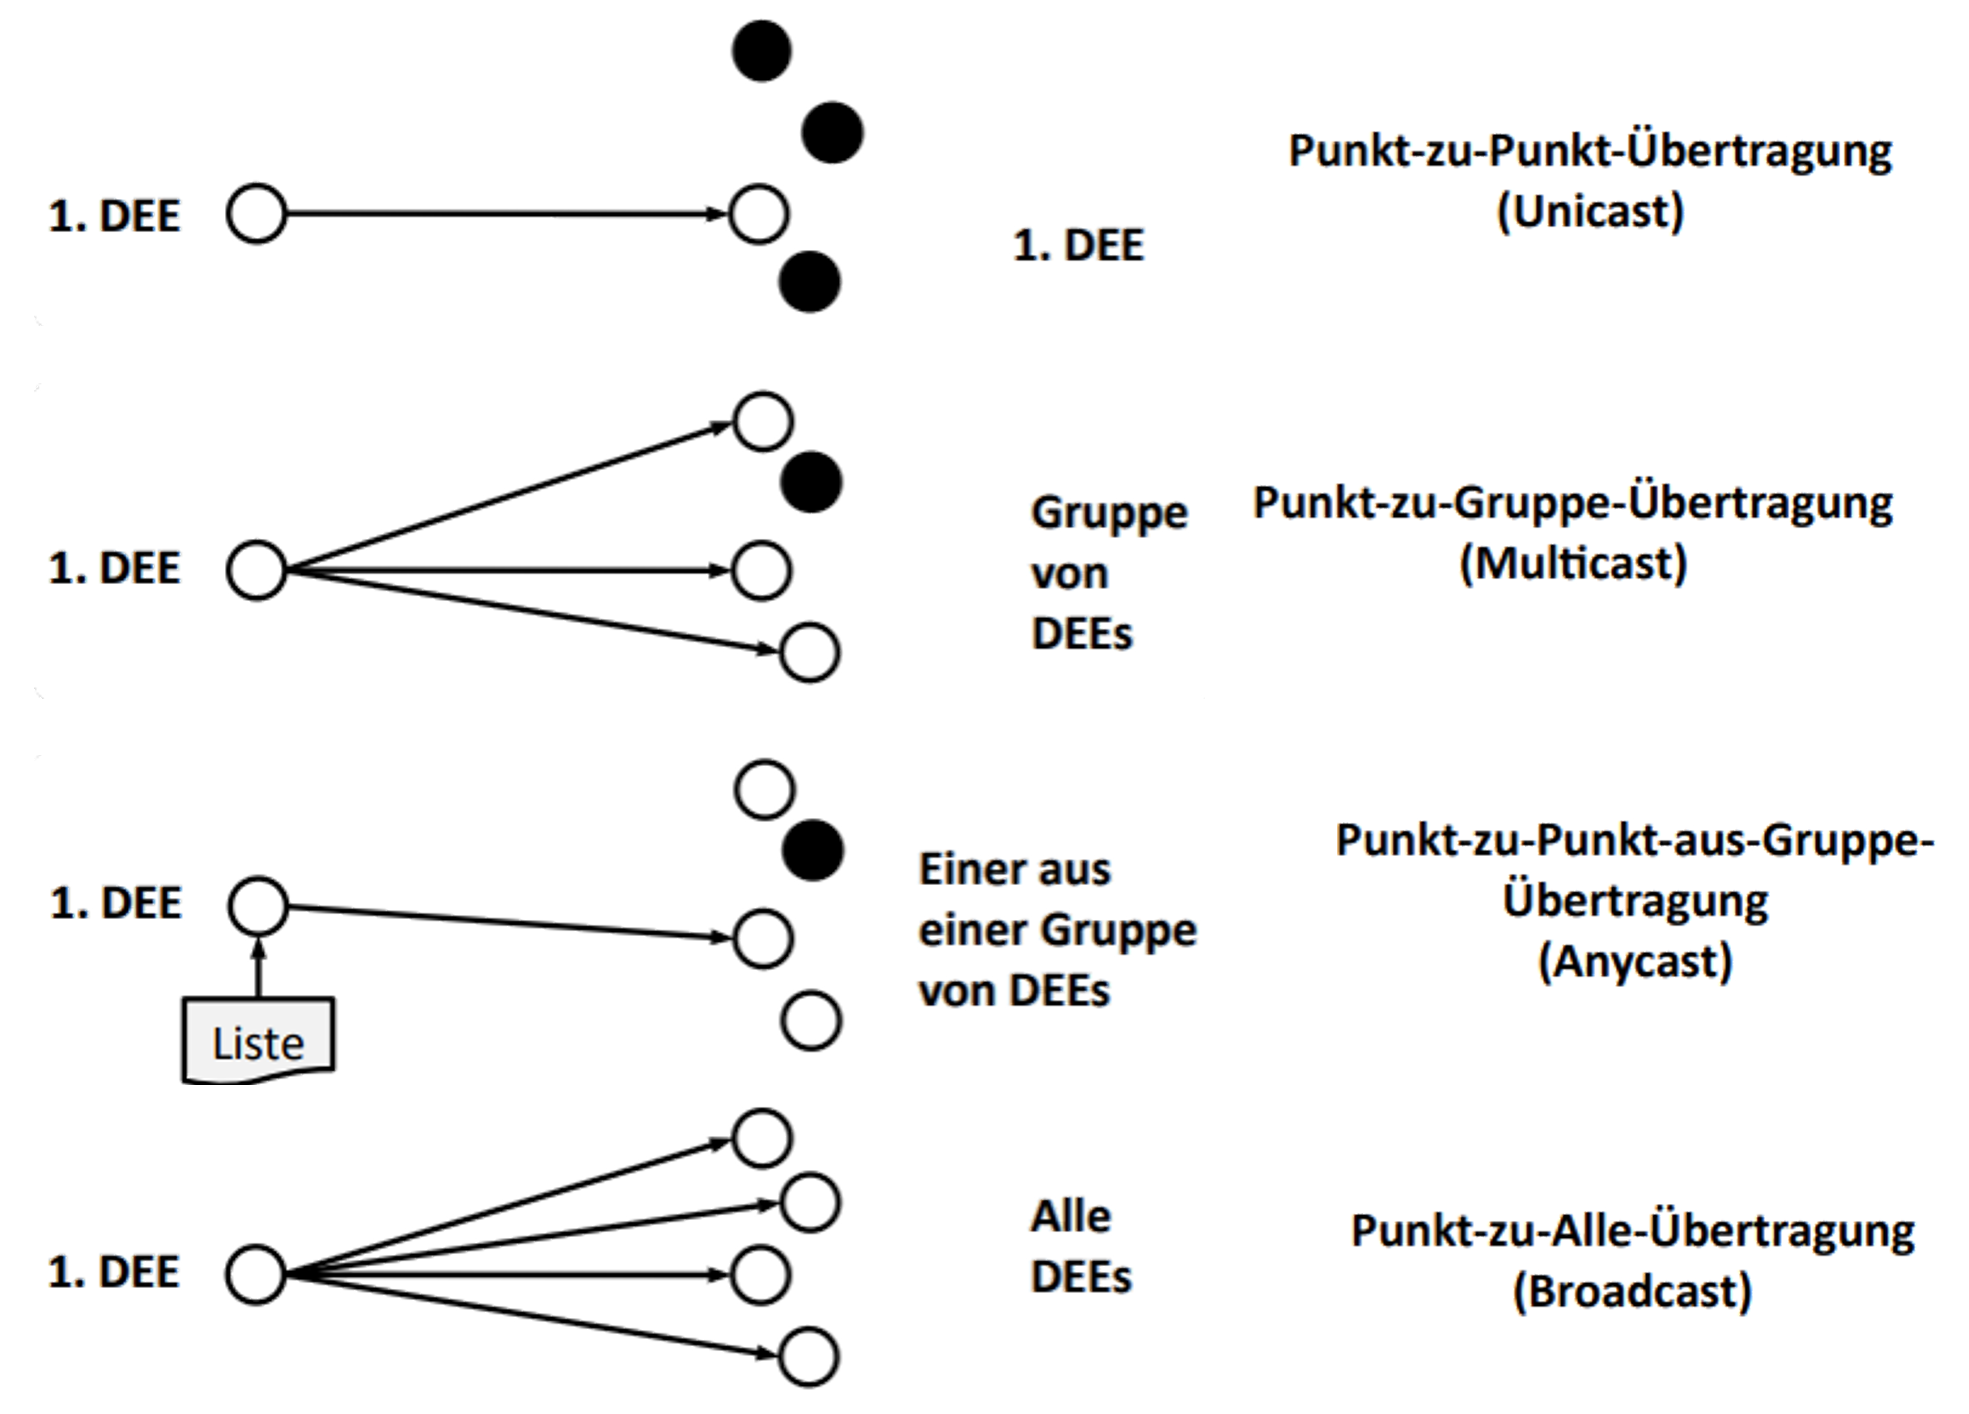
\includegraphics[width=\textwidth]{Bilder/Verkehrsarten.PNG}

		\subsection{Betriebsarten}
			\begin{center}
				\begin{figure}[!h]
					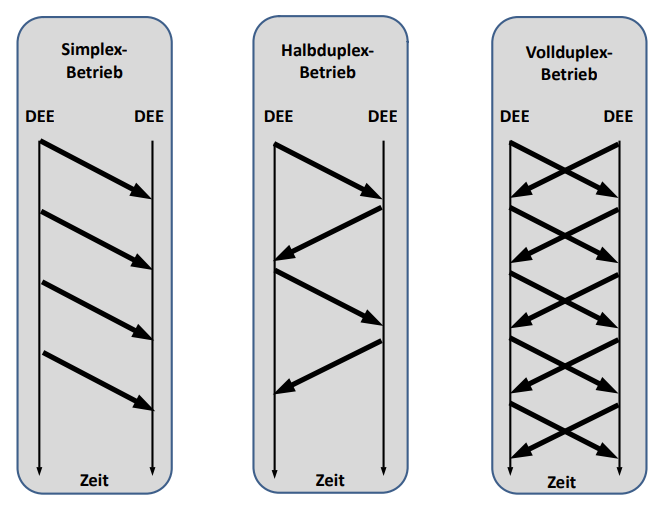
\includegraphics[scale=1]{Bilder/Duplexarten.PNG}
				\end{figure}
			\end{center}

		\subsection{Kabelarten:}
		\begin{description}
			\item[Twisted-Pair: ] Verdrillte Paare, um geringes Nebensprechen mit hoher Übertragbarkeit zu erreichen.
			\item[LWL: ] Lichtwellenleiter/Glasfaserkabel hohe Geschwindigkeit, teuer, Aufwand in Spannung zurückzuwandeln.  
		\end{description}

		\subsection{Ethernet-Standards}
		\begin{description}
			\item[10BaseT: ] 10 Mbit/s Twisted-Pair Kabel mit 100m Reichweite
			\item[10BaseF: ] 10 Mbit/s LWL (Fiber) mit 2000m Reichweite 
			\item[100BaseTX: ] 100 Mbit/s Twisted-Pair Kabel, durch Vollduplex-Übertragung
			\item[100BaseFX: ]  100 Mbit/s LWL, durch Vollduplex-Übertragung
			\item[RJ-45-Buchsen: ] Port für Netzwerkkarte mit 8 Pins
		\end{description}

		\subsection{Verkablungsarten:}
		\begin{description}
			\item[Primarverkabelung: ] Für Verkabelung von Gebäuden mit LWL
			\item[Sekundärverkabelung: ] Für Verkabelung von Etagen mit LWL
			\item[Tertiärverkabelung: ] Für Verkabelung innerhalb einer Etage mit Kupferkabel
		\end{description}
	
		\subsection{Informationskapazität}
		\begin{center}
			\begin{figure}[!h]
				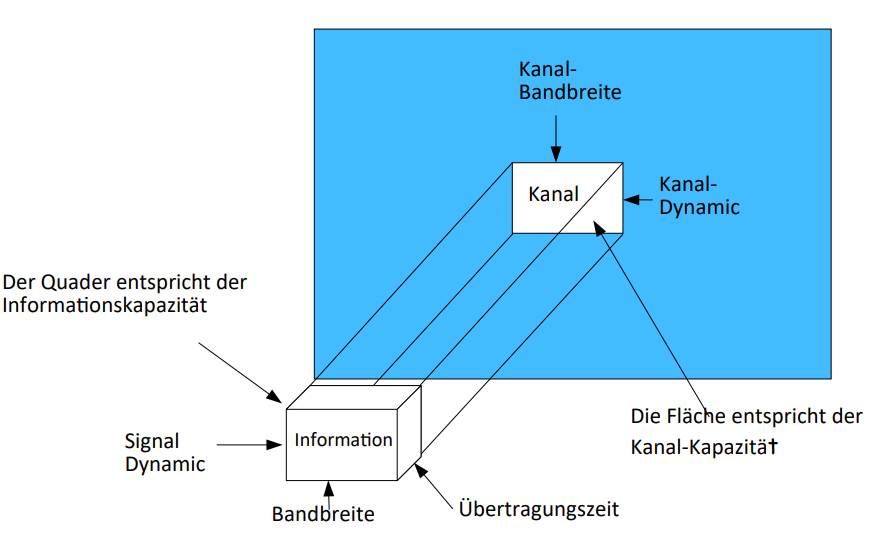
\includegraphics[width=\textwidth]{Bilder/Informationskapazitaet.png}
			\end{figure}
		\end{center}
		\begin{description}
			\item[Kanal-Bandbreite: ] Die Kanalbandbreite eines drahtlosen Signals bestimmt die Datenrate dieses Signals. Je höher die Kanalbandbreite, desto schneller ist die Verbindung. Die Verwendung einer Kanalbandbreite von160 MHz ist eines der Hauptmerkmale des neuen WLAN-Standards Wi-Fi 6.
			\item[Kanal-Dynamic: ] \textcolor{red}{Keine Ahnung?}
		\end{description}

		\subsection{Leitungstheorie}
			Um Leitungen vor elektromagnetischer Strahlung zu schützen, werden diese verdrillt. Je enger diese verdrillt werden, desto langsamer wird die Leitung(da der Weg länger wird).
			\begin{center}
				\begin{figure}[!h]
					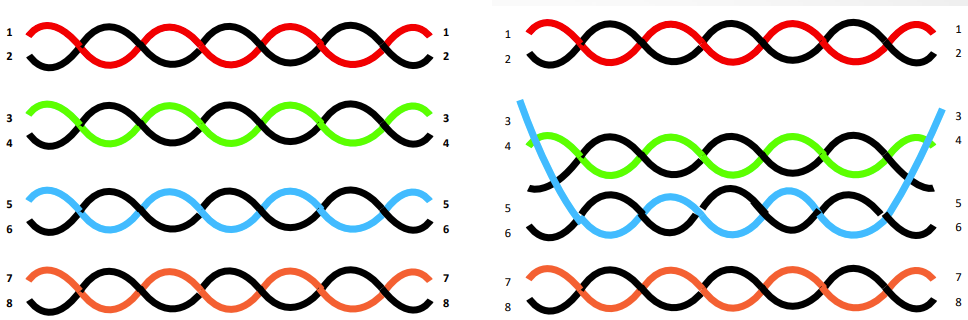
\includegraphics[width=\textwidth]{Bilder/verdrillte-kabel.PNG}
					Split Pairs \hspace{0.4\textwidth} Richtige Verdrahtung
				\end{figure}
			\end{center}
		

	\section{Satelliten}
	\begin{center}
		\begin{figure}[!h]
			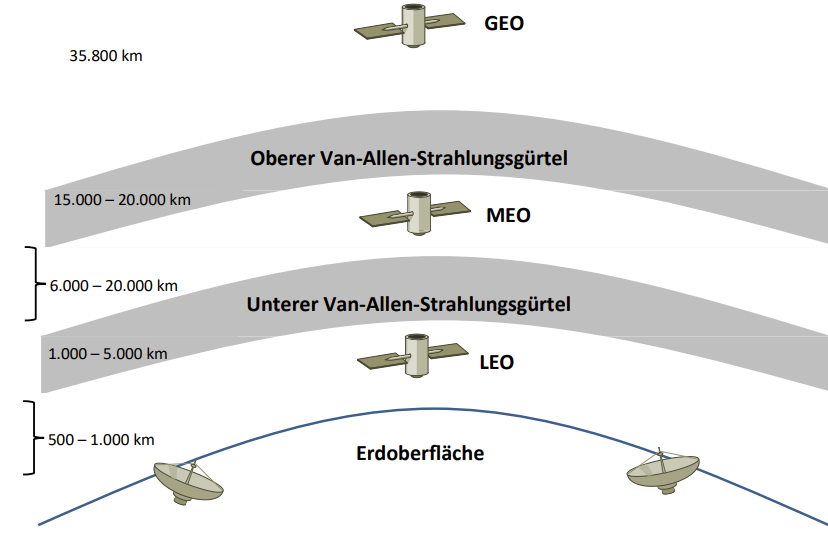
\includegraphics[width=\textwidth]{Bilder/Satelliten.png}
		\end{figure}
	\end{center}

	\section{Netze}
		\subsection{Netzwerk-Technologien}
			\begin{description}
				\item[Repeater] Verstärkt Eingangssignal auf Ausgang, OSI-Schicht 1
				\item[Hub] Multiport Repeater, OSI-Schicht 1
				\item[Bridge] Verbindet 2 Netze, arbeitet mit MAC-Adressen, OSI-Schicht 2 
				\item[Switch] Schlauer Hub. Verstärkt nur an richtigen Port. Arbeitet mit MAC-Adressen, OSI-Schicht 2 
				\item[Router] Verbindet Netze, arbeitet mit IP-Adressen, OSI-Schicht 3
				\item[Gateway] Verbindet Netze, arbeitet auf allen OSI-Schichten, Protokollunabhängig 
			\end{description}

		\subsection{Switch}
			\subsubsection{Spanning Tree}
				Switche haben Hierarchie beim Weiterleiten von Paketen. Kleine Priorität ist besser. Falls Priorität gleich, entscheidet höhere MAC-Adresse die bevorzugte Switch\\
				Switche geben Pakete nur an Switche mit geringerer Priorität oder höherer MAC-Adresse weiter. Beste Switch in der Vernetzung wird zum Root.\\
				Es gibt dabei 3 Arten von Ports an den Switches:
				\begin{description}
					\item[Root-Port] Zur Root-Switch
					\item[Designated-Port] Zu Switch mit besserer Priorität oder höherer MAC-Adresse als die eigene
					\item[Blocking-Port] Zu Switches, welche weniger bevorzugt sind als sie selbst 
				\end{description}
				In Untenstehender Skizze ist Switch B die Root-Switch und alle Ports, die zu ihr führen, sind Root-Ports.\\
				Da die restlichen Switche die gleiche Priorität haben, wird die höchste MAC-Adresse bevorzugt. \\
				Dadurch sind die Ports zu Switch A die Blocking-Ports und die von D zu A und C ebenfalls. \\
				Ports an Root-Switch sind alle designated.\\
				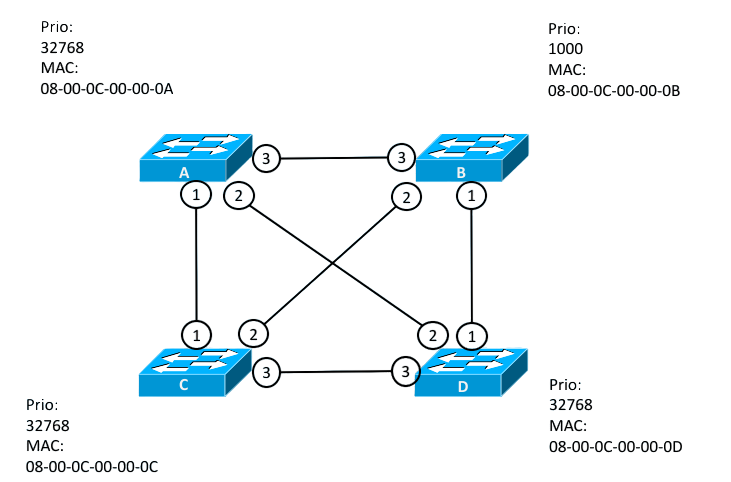
\includegraphics[width=\textwidth]{Bilder/RouterVermascht.png}

		\subsection{Netz Topologien}
			\begin{minipage}[t]{.48\textwidth}
				\begin{flushleft}
					\textbf{Baum Topologie}\newline\newline
					\begin{tikzpicture}[scale=0.8]
						\draw (-0.5,-0.5)rectangle(0.5,0.5);
						\draw (-3.5,-1.5)rectangle(-2.5,-0.5);
						\draw (2.5,-2.5)rectangle(3.5,-1.5);
						\draw (-3.5,-4.5)rectangle(-2.5,-3.5);
						\draw (-0.5,-5.5)rectangle(0.5,-4.5);
						\draw (2.5,-3.5)rectangle(3.5,-4.5);
						\draw[red] (-2.5,-1)--(-0.5,0);
						\draw[red] (-2.5,-4)--(0,-0.5);
						\draw[red] (2.5,-2)--(0,-0.5);
						\draw[red] (3,-2.5)--(0.5,-5);
						\draw[red] (3,-2.5)--(3,-3.5);
					\end{tikzpicture}\newline
					\footnotesize Vorteile:
					\begin{itemize}
						\footnotesize
						\item Bei Ausfall einer Komponente bricht nur ein Teil des Netzes zusammen
						\item leichte Skalierbarkeit
					\end{itemize}
					\footnotesize Nachteile:
					\begin{itemize}
						\footnotesize
						\item Durchsatzproblem an der Wurzel / jeder Netzkomponente $\longrightarrow$ höhere Laufzeiten
					\end{itemize}
				\vspace{0.3cm}
				{\normalsize\textbf{Bus-Topologie}}\newline\newline
					\begin{tikzpicture}[scale=0.8]
						\draw (-0.5,-0.5)rectangle(0.5,0.5);
						\draw (-3.5,-1.5)rectangle(-2.5,-0.5);
						\draw (2.5,-2.5)rectangle(3.5,-1.5);
						\draw (-3.5,-4.5)rectangle(-2.5,-3.5);
						\draw (-0.5,-5.5)rectangle(0.5,-4.5);
						\draw (2.5,-3.5)rectangle(3.5,-4.5);
						\draw (-2,0)--(2,-5);
						\draw (-1.9,0)--(2.1,-5);
						\draw (-2.5,-1)--(-1.2,-1);
						\draw (-2.5,-4)--(-0.4,-2);
						\draw (0,-0.5)--(0,-2.4);
						\draw (0,-4.5)--(0.4,-3);
						\draw (0.3,-2.8)--(2.5,-2);
						\draw (1.7,-4.5)--(2.5,-4);
					\end{tikzpicture}\newline
				\footnotesize Vorteile:
					\begin{itemize}
						\footnotesize
						\item hohe Ausfallsicherheit
						\item leichte Skalierbarkeit
					\end{itemize}
				\footnotesize Nachteile:
					\begin{itemize}
						\footnotesize
						\item Ausfall der Hauptleitung\newline $\longrightarrow$ Totalausfall
						\item Hauptleitung benötigt hohe Bandbreite
					\end{itemize}
				\end{flushleft}
			\end{minipage}
			\begin{minipage}[t]{.48\textwidth}
				\textbf{Stern Topologie}
				\begin{flushright}
					\begin{tikzpicture}[scale=0.8]
						\draw (-0.5,-0.5)rectangle(0.5,0.5);
						\draw (-3.5,-1.5)rectangle(-2.5,-0.5);
						\draw (2.5,-2.5)rectangle(3.5,-1.5);
						\draw (-3.5,-4.5)rectangle(-2.5,-3.5);
						\draw (-0.5,-5.5)rectangle(0.5,-4.5);
						\draw (2.5,-3.5)rectangle(3.5,-4.5);
						\draw (-0.5,-2)rectangle(0.5,-3);
						\draw[red] (-2.5,-1)--(-0.5,-2.5);
						\draw[red] (0,-0.5)--(0,-2);
						\draw[red] (-2.5,-4)--(-0.5,-2.5);
						\draw[red] (0,-3)--(0,-4.5);
						\draw[red] (0.5,-2.5)--(2.5,-2);
						\draw[red] (0.5,-2.5)--(2.5,-4);
					\end{tikzpicture}
				\end{flushright}
				\footnotesize Vorteile:
				\begin{itemize}
					\footnotesize
					\item Leicht umsetzbar / skalierbar
					\item sehr schnell
					\item Beim Ausfall einer Komponente ist \textit{nur} diese betroffen
				\end{itemize}
				\footnotesize Nachteile:
				\begin{itemize}
					\footnotesize
					\item Beim Ausfall der zentralen Wurzel\newline $\longrightarrow$ Totalausfall
					\item Clients müssen immer über zentrale Wurzel kommunizieren.
				\end{itemize}
				\vspace{0.3cm}
				{\normalsize\textbf{Ring-Tropologie}}\newline\newline
				\begin{flushright}
					\begin{tikzpicture}[scale=0.8]
						\draw (-0.5,-0.5)rectangle(0.5,0.5);
						\draw (-3.5,-1.5)rectangle(-2.5,-0.5);
						\draw (2.5,-2.5)rectangle(3.5,-1.5);
						\draw (-3.5,-4.5)rectangle(-2.5,-3.5);
						\draw (-0.5,-5.5)rectangle(0.5,-4.5);
						\draw (2.5,-3.5)rectangle(3.5,-4.5);
						\draw[red] (-2.5,-1)--(-0.5,0);
						\draw[red] (3,-1.5)--(0.5,0);
						\draw[red] (3,-2.5)--(3,-3.5);
						\draw[red] (3,-4.5)--(0.5,-5);
						\draw[red] (-3,-4.5)--(-0.5,-5);
						\draw[red] (-3,-3.5)--(-3,-1.5);
					\end{tikzpicture}
				\end{flushright}
				\footnotesize Vorteile:
				\begin{itemize}
					\footnotesize
					\item simpler Aufbau
					\item leichte Skalierbarkeit
					\end{itemize}
					\footnotesize Nachteile:
					\begin{itemize}
						\footnotesize
						\item Unterbrechung des Rings\newline $\longrightarrow$ Totalausfall
						\end{itemize}
			\end{minipage}
		
		\subsubsection{Netze in Unternehmen}
			Das Verwenden eines Netzes hat signifikante Vorteile für ein Unternehmen / Betrieb. Ressourcen und Betriebsmittel können gemeinsam genutzt werden (Zentral-Drucker). Dadurch können Kosten eingespart werden. Die Kommunikation innerhalb des Unternehmens wird durch verschiedene Netze (internes Telefon, Kommunikation zwischen den Systemen) um ein vielfaches erleichtert. Sollte das Unternehmen im Laufe der Zeit an Größe zulegen, ist die Skalierbarkeit des Systems im Allgemeinen unbegrenzt. Zusätzliche Systeme oder Server können problemlos hinzugefügt werden. Die Systemleistung eines einzelnen Computers kann außerdem gesteigert werden. Aufwendige Anwendungen können auf einem leistungsstarken Server ausgeführt werden, sind also nicht an die locale Leistung eines einzelnen Computers gebunden. Die Komponente der Teamarbeit im globalen Sinne wird durch ein globales Netzwerk zwischen Unternehmen außerdem vereinfacht.
		
		\subsubsection{Private Netze}
			Besitzt ein Haushalt einen Home Server mit Internetanbindung, so ist es Privatpersonen möglich, von nahezu überall auf der Welt auf ihre persönlichen Daten zugreifen zu können. Diese Option steht Privatpersonen außerdem durch Cloud Services zur Verfügung. Nachteil: Die Daten werden externen Firmen zur Verfügung gestellt, diese Option ist mit Vorsicht zu genießen. Privatpersonen können durch das Internet außerdem auf, generell betrachtet, Online Services zugreifen (Online Banking, Online Shopping). Die Kommunikation wird auch für Privatpersonen erheblich erleichtert. Durch Chat, Voice Chat oder sogar Video Chat Anwendungen ist die Kommunikation nahezu an jedem Ort der Erde möglich. Auch das Unterhaltungsprogramm profitiert vom Internet. Dienste wie YouTube oder Netflix wären ohne das Internet undenkbar.
		
		\subsection{Servermodelle}
		\begin{table}[h]
			\renewcommand{\arraystretch}{1.5}	
			\centering
				\begin{tabularx}{17cm}{|X|X|}
					\hline
					\cellcolor{cyan!60!white}Art&\cellcolor{cyan!60!white}Beschreibung\\
					\hline
					Ein-Server-Modell&Ein Computer/Server übernimmt alle zentralen Dienste \\
					\hline
					Mulit-Server-Modell&Mehrere Computer/Server teilen sich die Verwaltung (für große Netze) \\
					\hline
				\end{tabularx}
		\end{table}
		
		\subsection{Kommunikationsarten}
		\begin{table}[h]
			\renewcommand{\arraystretch}{1.5}	
			\centering
				\begin{tabularx}{17cm}{|X|X|}
					\hline
					\cellcolor{cyan!60!white}Art&\cellcolor{cyan!60!white}Beschreibung\\
					\hline
					Simplex&Einer spricht, der Rest hört zu \\
					\hline
					Halbduplex&Wechselseitiges Sprechen und Hören \\
					\hline
					Vollduplex& Jeder spricht und hört gleichzeitig \\
					\hline
				\end{tabularx}
		\end{table}
		
		\subsection{Netzwerkkomponenten}
		\subsubsection{Port}
			Ein Port ist der Teil einer Netzwerk-Adresse, der die Zuordnung von TCP- und UDP-Verbindungen und -Datenpaketen zu Server- und Client-Programmen durch Betriebssysteme bewirkt. Zu jeder Verbindung dieser beiden Protokolle gehören zwei Ports, je einer auf Seiten des Clients und des Servers.
		
		\subsubsection{Client}
			Der Client stellt einen Rechner im Netz dar. Er simuliert einen Computer an einem gewissen Standpunkt. Der Client besitzt eine Network-Interface-Card.
			\begin{center}
				\begin{tikzpicture}
						\draw[black](-1.4, -1) rectangle (1.4,1);
						\draw[black](-1.1, -0.8) rectangle (1.1,0.8);
						\node at (0,0){\textbf{Client}};
				\end{tikzpicture}
			\end{center}
		
		\subsubsection{Netzwerkkarte}
			Eine Netzwerkkarte besitzt eine individuelle MAC-Adresse und befindet sich in eigentlich jedem Rechner. Sie stellt die Verbindung zwischen dem Rechner und dem Netzwerkmedium dar. Außerdem verfügt sie über eine Netzwerk-Schnittstelle.
		
		\subsubsection{Repeater}
			Der Repeater hat jeweils einen Eingang und einen Ausgang. Er verstärkt Signale durch regenerieren/synchronisieren des Taktes. Dazu arbeitet er auf Bitebene und verursacht eine kleine Latenz.
				\begin{center}
					\begin{tikzpicture}
						\draw[black](-1.4, -1) rectangle (1.4,1);
						\draw [<->, black, very thick](-1,0) to(1,0);
					\end{tikzpicture}
				\end{center}
		
		\subsubsection{HUB}
		Der HUB ist ein Multiport Repeater. D.h. er hat mehrere Ein- und Ausgänge und arbeitet auch auf Bitebene.
				\begin{center}
					\begin{tikzpicture}
						\draw[black](-1.4, -1) rectangle (1.4,1);
						\draw [<->, black, very thick](-1,0) to(1,0);
					\end{tikzpicture}
				\end{center}
		
		\subsubsection{Bridge}
			Die Bridge fungiert als Brücke zwischen zwei LAN-Netzwerken. Sie kennt die relevanten MAC-Adressen in beiden Netzen und verbindet so die Netze miteinander.
				\begin{center}
					\begin{tikzpicture}
						\draw[black](-1.4, -1) rectangle (1.4,1);
						\draw [->, black, very thick](-1,0.2) to(-0.2,0.2);
						\draw [->, black, very thick](-1,-0.4) to(-0.2,-0.4);
						\draw [->, black, very thick](1,0.4) to(0.2,0.4);
						\draw [->, black, very thick](1,-0.2) to(0.2,-0.2);
					\end{tikzpicture}
				\end{center}
		
		\subsubsection{Switch}
			Der Switch ist eine Multiport-Bridge. D.h. er hat mehrere Ein- und Ausgänge und verbindet so mehrere Netzwerke miteinander. Er verwendet Filtertabellen um den schnellsten Weg für Signale zu finden. Er arbeitet ebenso mit MAC-Adressen.
				\begin{center}
					\begin{tikzpicture}
						\draw[black](-1.4, -1) rectangle (1.4,1);
						\draw [->, black, very thick](-1,0.2) to(-0.2,0.2);
						\draw [->, black, very thick](-1,-0.4) to(-0.2,-0.4);
						\draw [->, black, very thick](1,0.4) to(0.2,0.4);
						\draw [->, black, very thick](1,-0.2) to(0.2,-0.2);
					\end{tikzpicture}
				\end{center}
		
		\subsubsection{Router}
			Der Router verbindet Netzwerke indem er Datenpackete weiterleitet oder blockiert. Er arbeitet mit IP-Adressen und wird oft auch als intelligenter Switch bezeichnet. Der Router wird für das gesamte Netz verwendet.
				\begin{center}
					\begin{tikzpicture}
						\draw[black, very thick](0, 0) circle (1.6);
						\draw [->, black, very thick, line width=1mm](-1,1) to(-0.2,0.2);
						\draw [->, black, very thick, line width=1mm](1,-1) to(0.2,-0.2);
						\draw [->, black, very thick, line width=1mm](0.2, 0.2) to(1,1);
						\draw [->, black, very thick, line width=1mm](-0.2,-0.2) to(-1,-1);
					\end{tikzpicture}
				\end{center}
		
		\subsubsection{Einordnung der Komponenten ins OSI-Modell}
			Die Netzwerkkomponenten lassen sich in die Schichten 1 bis 4 einordnen. Die Schicht 1 beinhaltet alle Kabel(Kupferkabel, Ethernetkabel, Glasfaserkabel) und den Repeater. Zu Schicht 2 gehören Switches und Bridges. In Schicht 3 ist der Router und in Schicht 4 handelt es sich um die Netzwerkkarte und die Ports.
			\begin{center}
				\renewcommand{\arraystretch}{1.5}
					\begin{tabularx}{17cm}{|c|X|X|}
						\hline
						\cellcolor{cyan!60!white}\textbf{Nummer} & \cellcolor{cyan!60!white}\textbf{Bezeichnung} & \cellcolor{cyan!60!white}\textbf{Komponenten}\\
						\hline
						1 & Bitübertragungsschicht & Repeater, Kabel\\
						\hline
						2 & Sicherungsschicht & Switches, Bridges\\
						\hline
						3 & Vermittlungsschicht & Router\\
						\hline
						4 & Transportschicht & Netzwerkkarte, Ports\\
						\hline
					\end{tabularx}
			\end{center}
		
		\subsection{Round Trip Delay Time - RTDT}
			Die Paketumlaufzeit bzw. Round Trip Time gibt die Zeit an, die ein Datenpaket in einem Rechnernetz benötigt, um von der weitesten entfernten Quelle zum Ziel und zurück zu reisen. Es handelt sich also um die Summe aus Laufzeit von Punkt A nach Punkt B und der Laufzeit von Punkt B nach Punkt A.
				\begin{center}
					\begin{tikzpicture}
						\draw (-5,-3)rectangle(-3,-1);
						\draw (-5.5,-3.5)rectangle(-2.5,-0.5);
						\draw (-4,1)rectangle(-2,3);
						\draw (-4.5,0.5)rectangle(-1.5,3.5);
						\draw (0,-4)rectangle(2,-2);
						\draw (-0.5,-4.5)rectangle(2.5,-1.5);
						\draw (1,2)rectangle(3,4);
						\draw (0.5,1.5)rectangle(3.5,4.5);
						\draw (6,1)rectangle(8,3);
						\draw (5.5,0.5)rectangle(8.5,3.5);
						\draw[black] (-5,0)--(9,0);
						\draw[red, very thick](-4,0)--(7,0);
						\draw[red, very thick] (-4,-0.5)--(-4,0);
						\draw[red, very thick] (7,0)--(7,0.5);
						\draw[black] (-3,0)--(-3,0.5);
						\draw[black] (1,0)--(1,-1.5);
						\draw[black] (2,0)--(2,1.5);
						\node at (-4,-2){Client A};
						\node at (7,2){Client B};
						\draw [->, very thick, red](-0.5,0.5) to(0,0.5);
						\draw [->, very thick, red](0,-0.5) to(-0.5,-0.5);
					\end{tikzpicture}
				\end{center}
		
		\subsection{Bezeichnungen von Netzen}
			\begin{table}[h]
				\footnotesize
				\renewcommand{\arraystretch}{2}
				\begin{tabularx}{17cm}{|l|X|c|X|}
					\hline
					\cellcolor{cyan!60}Abkürzung&Beschreibung&Ausdehnung&Anwendungen\\
					\hline
					\cellcolor{cyan!30}BAN&Body Area Network&1m&Wearable Computers\\
					\hline
					\cellcolor{cyan!30}PAN&Personal\newline Area Network&10m&Bluetooth\\
					\hline
					\cellcolor{cyan!30}LAN&Local Area Network&10km&LAN/WLAN\\
					\hline
					\cellcolor{cyan!30}SAN&Storage Area Network&10km&für Datenspeicherung/-sicherung\\
					\hline
					\cellcolor{cyan!30}MAN&Metropolitan\newline Area Network&100km&Stadtgebiet\\
					\hline
					\cellcolor{cyan!30}WAN&Wide Area Network&mehrere 1.000km&Öffentliche Netze(LTE, 5G, ...)\\
					\hline
					\cellcolor{cyan!30}GAN&Global Area Network&mehrere 10.000km&Erdumspannende Netze die WAN's über Satelliten und Seekabel miteinander verbinden\\
					\hline
				\end{tabularx}
			\end{table}
		
		\section{Ethernet}
			Mit der Erfindung des Ethernets wollte man individuellen Stationen / Systemen den Zugriff auf ein gemeinsames Medium zur Datenübertragung ermöglichen. Die Netzwerktechnologie verwendet das CSMA/CD Verfahren und eignet sich primär für lokale Netze.
			\begin{figure}[h]
				\centering
				\begin{tikzpicture}
					\draw[black, very thick] (-1,0) rectangle (1,2);
					\draw[black, very thick] (-4,0) rectangle (-2,2);
					\draw[black, very thick] (2,0) rectangle (4,2);
					\node at (0,1){PC 10};
					\node at (-3,1){PC 01};
					\node at (3,1){PC 11};
					\draw[red, very thick] (-3,0)--(-3,-1);
					\draw[red, very thick] (0,0)--(0,-1);
					\draw[red, very thick] (3,0)--(3,-1);
					\draw[red, very thick] (-5,-1)--(5,-1);
					\draw[black, very thick] (-6,-0.5) rectangle (-5,-1.5);
					\draw[black, very thick] (6,-0.5) rectangle (5,-1.5);
					\node at (-7,-1){Absorber};
					\node at (7,-1){Absorber};
					\node at (0,-1.5){Koax. Kabel};
				\end{tikzpicture}
			\end{figure}\newline
			Soll ein Datenpaket verschickt werden (z.B. ein Zahlenwert), so muss der Sender das Ziel des Paketes kennen, um die Information zum korrekten Empfänger schicken zu können. \newline
			Will \textit{PC 01} die Zahl \textit{5d} an \textit{PC 10} senden, ergibt sich folgender Rahmen:
			\begin{center}
				\begin{tabularx}{14cm}{|X|X|}
					\hline
					0010 \textit{(Kennung des Ziels, 4Bit)}&0101 \textit{(Daten, 4Bit)}\\
					\hline
				\end{tabularx}
			\end{center}
			Damit der Empfänger den Erhalt der Daten quittieren kann, muss jedoch auch die Kennung des Senders im Rahmen enthalten sein:
			\begin{center}
				\begin{tabularx}{17cm}{|X|X|X|}
					\hline
					0010 \textit{(Kennung des Ziels)}&0001 \textit{(Kennung der Quelle)}&0101 \textit{(Daten)}\\
					\hline
				\end{tabularx}
			\end{center}
			Der verschickte Rahmen lautet demnach:
			\begin{center}
				\begin{tabularx}{5cm}{XXX}
					0010&0001&0101\\
				\end{tabularx}
			\end{center}
			Um zu wissen, ob es sich bei den empfangenen Impulsen tatsächlich um eine gesendete Information handelt, wird ein Datenrahmen immer durch eine Präambel angekündigt. Es könnten sonst Missverständnisse durch Signalrauschen oder Störungen auftreten. Die endgültige Struktur eines Datenrahmens:
			\begin{center}
				\begin{tabularx}{17cm}{|l|l|X|X|X|}
					\hline
					Präambel (7Byte)&SFD (1Byte)&Ziel (MAC)&Quelle (MAC)&Nutzdaten\\
					\hline
				\end{tabularx}
			\end{center}
		   
		\subsection{Vollständiges Ethernet-Paket}
			\begin{center}
				\renewcommand{\arraystretch}{1.5}
				\begin{tabularx}{17cm}{|l|l|l|X|X|X|r|}
					\hline
					Präambel 7&SFD 1&Ziel-Mac 6&Quell-MAC 6&Typ 2&Nutzdaten 46-1500&CRC 4\\
					\hline
				\end{tabularx}
			\end{center}
			\begin{center}
				Zahlenwert im Feld = Bytegröße des Feldes.
			\end{center}

		\subsection{Ethernet-Synchronisation}
			Um das Signal bei einer Übertragung zu synchronisieren wird vor jedem Ethernetframe eine Präambel und ein SFD(Start Frame Delimiter) gepackt. Die Präambel lautet \textit{1010101010...} für 7 Byte und der SFD ist 1 Byte groß: \textit{10101011}.
		
	\section{Zugriffsverfahren}
		Bei geteilten Medium wird ein Zugriffsverfahren benötigt(außer Switch). Folgende Zugriffsverfahren stehen zur Auswahl:
		
		\subsection{ALOHA}
			\begin{center}
				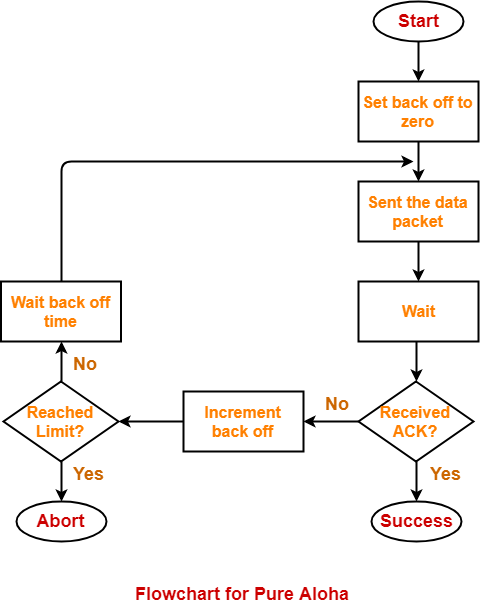
\includegraphics[width=0.6\textwidth]{Bilder/aloha.png}
			\end{center}

		\subsection{CSMA}
			\begin{center}
				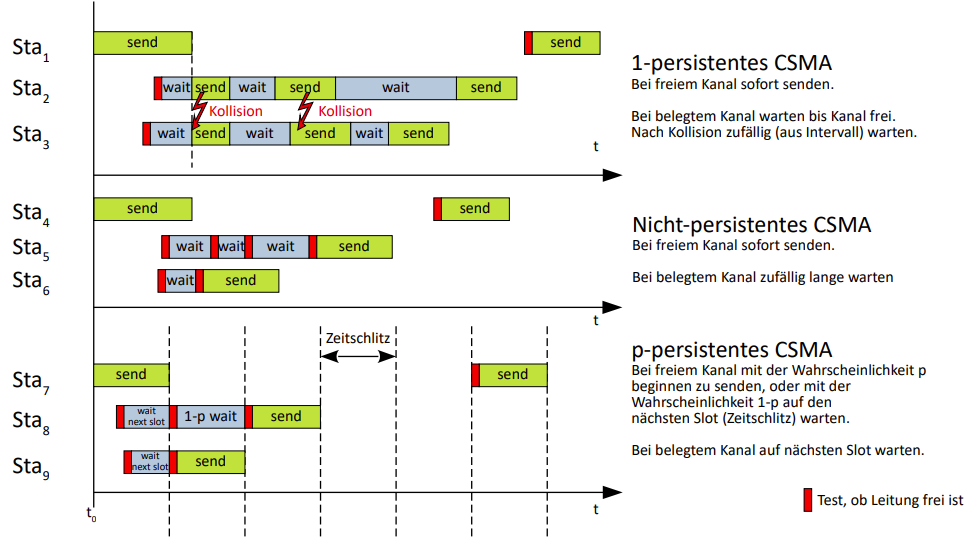
\includegraphics[width=\textwidth]{Bilder/csma.PNG}
			\end{center}

		\subsection{CSMA/CA}
			\begin{center}
				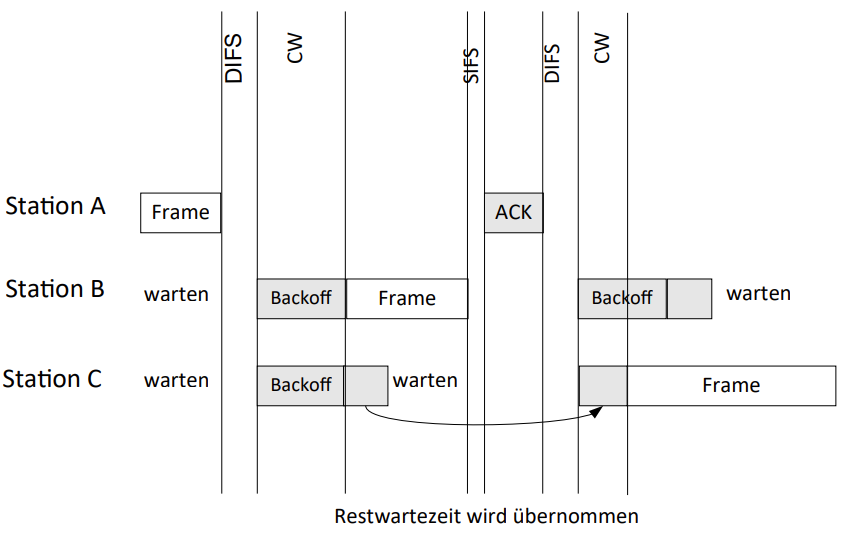
\includegraphics[width=\textwidth]{Bilder/csmaca.PNG}
			\end{center}

		\subsection{CSMA/CD - Verfahren}
			Programmablaufplan des CSMA/CD Verfahrens:
			\begin{center}
				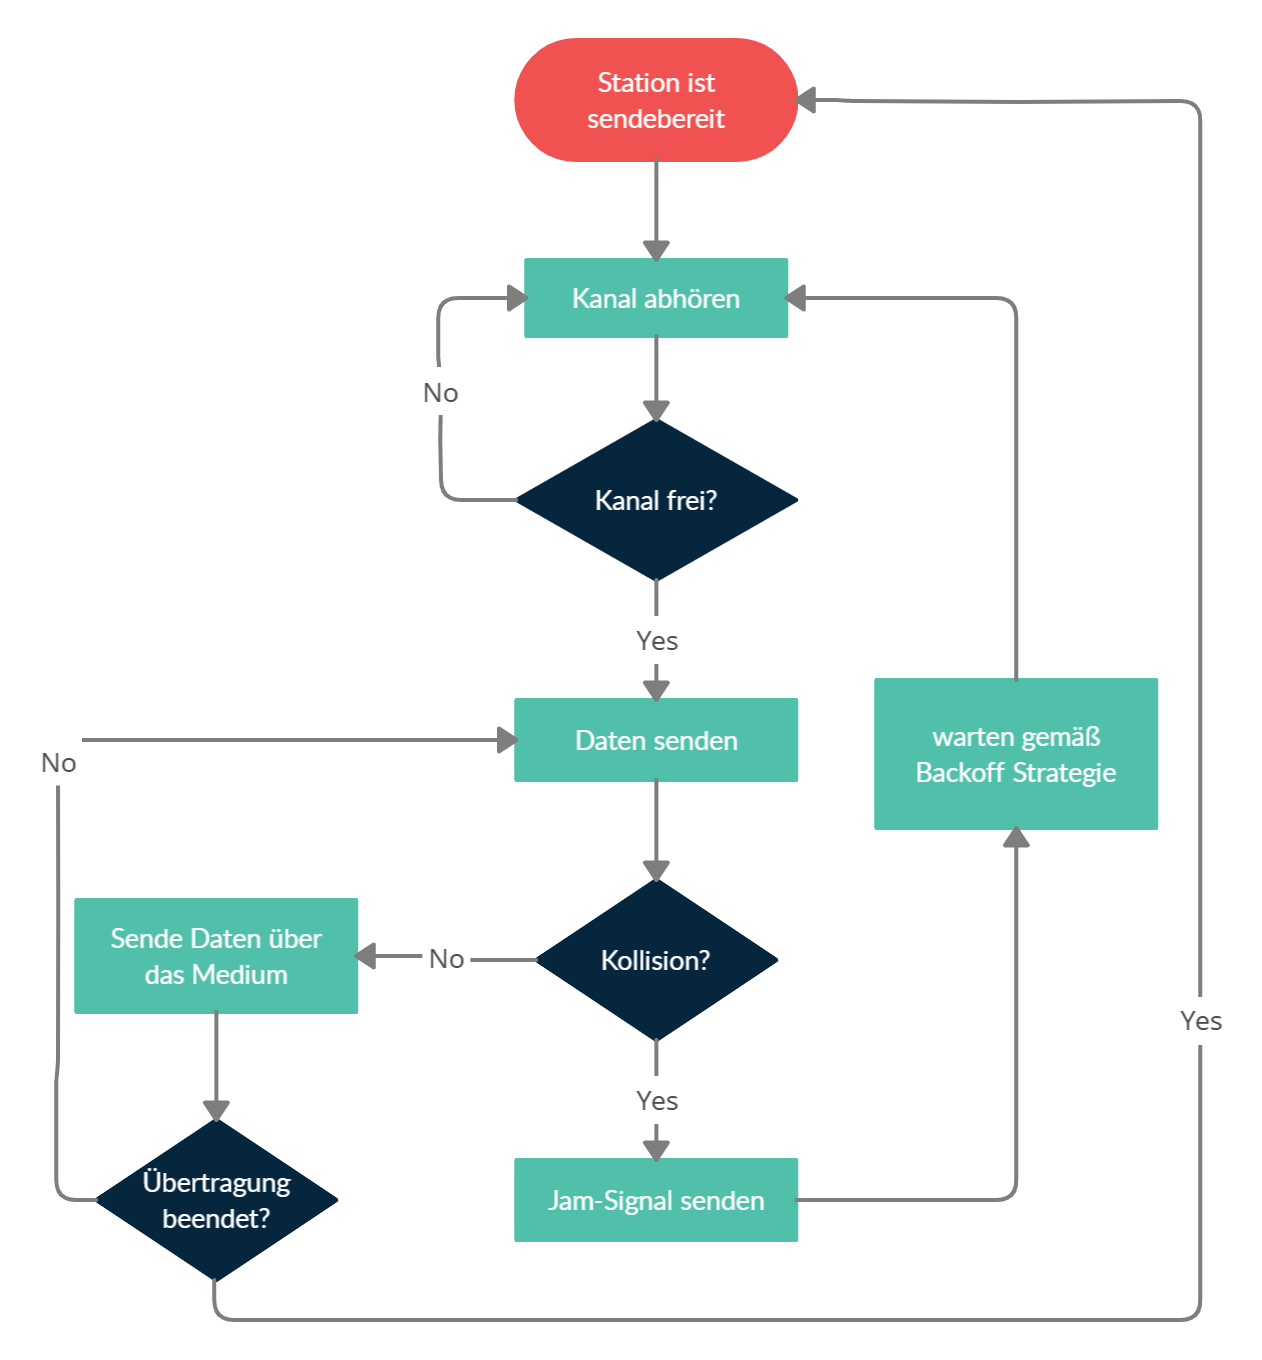
\includegraphics[width=0.6\textwidth]{Bilder/CSMACD.png}
			\end{center}
		
		\subsubsection{Kollision}
			\textbf{Problem:}\newline 
			Da Alle Systeme mit nur einem Übertragungsmedium vernetzt sind, um Materialkosten zu sparen, und Skalierbarkeit zu erhalten, muss der Leiter bidirektional verwendet werden. Dadurch kann es zu Kollisionen von Impulsen kommen.\newline
			$\longrightarrow$ Es kommt zu einer Signalerhöhung / Signalverbreiterung und damit zu einer fehlerhaften Übertragung.\newline\newline
			\textbf{Lösung:}\newline
			CSMA/CD Verfahren - Jam Signal
			\noindent\textbf{Situation:}
			\begin{center}
				\begin{tikzpicture}
					\draw[black, very thick](-7,-1)rectangle(-5,1);
					\draw[black, very thick](7,-1)rectangle(5,1);
					\draw[red, very thick](-5,0)--(5,0);
					\node at (-6,0){PC};
					\node at (6,0){PC};
					\filldraw[fill=green!50,draw=black,very thick](-4.5,0)rectangle(-3.5,1);
					\filldraw[fill=green!50,draw=black,very thick](-2,0)rectangle(0,1);
					\filldraw[fill=blue!50,draw=black,very thick](3,0)rectangle(3.5,1);
					\filldraw[fill=blue!50,draw=black,very thick](1,0)rectangle(2,1);
					\draw[->,black, very thick](-4.5,-0.5)--(-2,-0.5);
					\draw[->,black, very thick](4.5,-0.5)--(2,-0.5);
		
					\draw[black, very thick](-7,-2)rectangle(-5,-4);
					\draw[black, very thick](7,-2)rectangle(5,-4);
					\draw[red, very thick](-5,-3)--(5,-3);
					\node at (-6,-3){PC};
					\node at (6,-3){PC};
					\filldraw[fill=green!50,draw=black,very thick](-2.5,-3)rectangle(-1.5,-2);
					\filldraw[fill=green!50,draw=black,very thick](0,-3)rectangle(2,-2);
					\filldraw[fill=blue!50,draw=black,very thick](1,-2)rectangle(1.5,-1);
					\filldraw[fill=blue!50,draw=black,very thick](-1,-3)rectangle(0,-2);
					\draw[red, very thick](0.8,-0.8)rectangle(1.7,-3.2);
					\draw[red, very thick](-1.2,-3.2)rectangle(0.2,-1.8);
					\node at (2.2,-3.7){Signalerhöhung};
					\node at (-2,-3.7){Signalverbreiterung};
				\end{tikzpicture}
			\end{center}
			Das sendende System vergleicht ständig das gesendete Signal mit dem Signal auf der Leitung. Kommt es zu Abweichungen bricht das System die Übertragung ab und sendet ein Jam-Signal welches andere Systeme im Netz über die Kollision informiert. Alle Systeme unterbrechen die Übertragung.\newline
			Ab wann dürfen die einzelnen Systeme wieder anfangen Daten zu senden?\newline\newline
			Jedes Signal auf der Leitung braucht eine bestimmte Zeit, um zwischen den beiden entferntesten Systemen im Netz einmal hin, und wieder zurück zu laufen. Diese Zeit wird mit RTT bezeichnet. Ist die RTT abgelaufen, befinden sich keine Signale mehr im Netz, es kann neu gesendet werden. \newline\newline
			Nach dem Ethernet-Standard 802.3 ist die RTT auf 51,2 Mikrosekunden festgelegt.\newline\newline
			Kommt es nach dem Warten der RTT dennoch zu einer weiteren Kollision, variieren die Systeme ihre Wartezeit indem sie ein vielfaches der RTT warten. Als Vielfaches können die Faktoren 0,1,2 und 3 gewählt werden.\newline
			$\longrightarrow$ Es wird unterschiedlich lang gewartet. \newline\newline
			Kommt es erneut zu einer Kollision, wird der Bereich der Vorfaktoren von 0 bis 7 erweitert.
			\begin{center}
				Wartezeit= k $\cdot$ RTD
			\end{center}
			\begin{center}
				k = 0 bis $2^{i}$-1 \hspace{2cm} i = Anzahl Versuche
			\end{center}
			Nach 10 Versuchen wird i nicht mehr erhöht, nach 16 erfolglosen Versuchen wird der Sendeversuch abgebrochen.

		\subsection{Token Ring}
			Bei Token Ring wird ein sog. Token im Kreis gelassen. An diesen heftet jeder Client seine Nachrichten an und und liest die für ihn vorgesehene Nachrichten. Der Token durchläuft hierbei die Staten \textit{frei}, \textit{belegt} und \textit{gelesen}. Somit wird der Token erst wieder freigegeben, wenn der Sender die Rückmeldung gelesen erhalten. \textcolor{red}{Wenn der Token nicht gelesen wurde und der Sender die Nachricht ungelesen zurück bekommt, wird dieser dann wieder frei? @flo und @ozan}
			
	\section{Netzwerkprotokolle}%Hier gerne noch andere Protokolle :)
			Hat die Netzwerkkarte einen Datenrahmen empfangen, muss ermittelt werden, welches Protokoll zur Weiterverarbeitung verwendet werden soll. Innerhalb des Datenrahmens muss also der Typ und das Ziel der Daten festgelegt sein. Diese Informationen stehen in einem 2Byte großem Typenfeld. Für jedes Protokoll existiert eine eigene Kennung:
			\begin{center}
				\renewcommand{\arraystretch}{1.5}
				\begin{tabularx}{10cm}{|X|X|}
					\hline
					ARP&0x0806\\
					\hline
					IPv4&0x0800\\
					\hline
					IPv6&0x86DD\\
					\hline
				\end{tabularx}
			\end{center}
			Allerdings kommt dem Typenfeld eine weitere Bedeutung:
			\begin{center}
				\renewcommand{\arraystretch}{1.5}
				\begin{tabularx}{14cm}{|X|X|}
					\hline
					Wert kleiner als 0x0600&Länge des Datenrahmens\\
					\hline
					Wert größer als 0x0600&Protokollkennung\\
					\hline
				\end{tabularx}
			\end{center}
			Alle Protokollkennungen müssen also größer als 1536d oder 0x0600h sein!\newline\newline
			\textbf{Achtung:}\newline
			Das ICMP Netzwerkprotokoll ist ein Protokoll der IP-Familie und folgt somit dem IPv4-Protokoll!\newline
			Ebenso gehört das ICMPv6 Netzwerkprotokoll zur IPv6 Familie und folgt somit auch dem IPv6 Protokoll!
		
		\subsection{Datenübertragung}
			Um sicher zu gehen, dass alle Informationen fehlerfrei übertragen wurden, wird dem Datenrahmen ein 4Byte großes Prüffeld (CRC) angehängt. Dieses Prüffeld ergibt sich aus einer Polynomdivision.
			\begin{center}
				\renewcommand{\arraystretch}{1.5}
				\begin{tabularx}{17cm}{|l|l|X|X|X|X|r|}
					\hline
					Präambel&SFD&Ziel-Mac&Quell-MAC&Typ&Nutzdaten&CRC\\
					\hline
				\end{tabularx}
			\end{center}
			\begin{tikzpicture}[remember picture,overlay,thick,black,shorten <=1pt,shorten >=1pt]
				\begin{scope}[c/.style={shift={(-\tabcolsep,\the\dimexpr\fontdimen22\textfont2\relax)}}]
					\draw(3.55,0)--(17,0);
					\draw(3.55,0.5)--(3.55,0);
					\draw(17,0.5)--(17,0);
					\node at (10,-0.5){Min: 64Byte - Max: 1518Byte};
				\end{scope}
			\end{tikzpicture}\newline\newline\newline
			Unterschreitet der Anteil der Nutzdaten 46Byte, wird durch Padding aufgefüllt.
		
		\newpage
		
		\section{ARP-Protokoll}
			Programmablaufplan des ARP Verfahrens:
			\begin{center}
				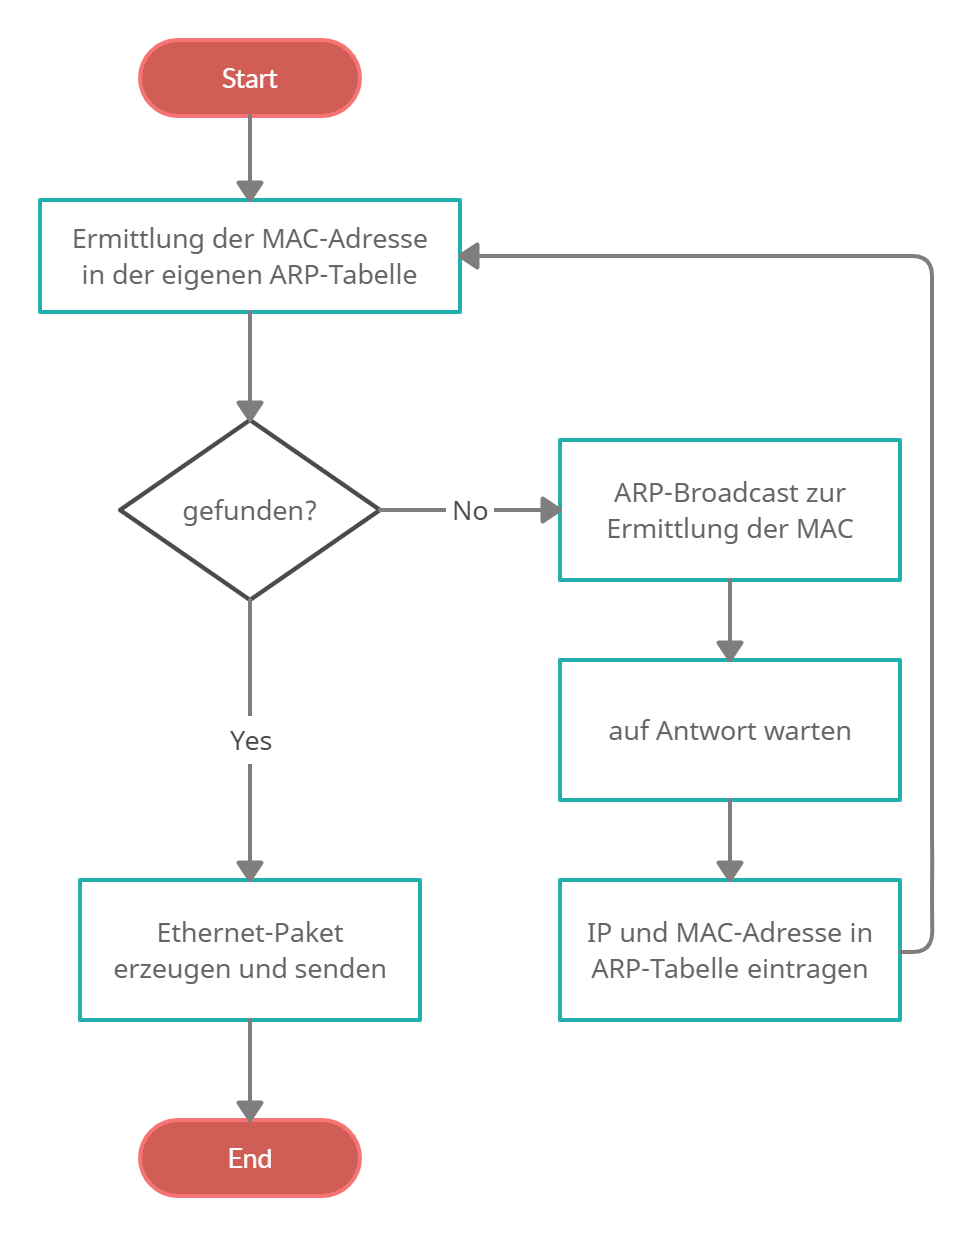
\includegraphics[scale=0.3]{Bilder/ARP-Protokoll PAP.png}
			\end{center}
		
		\section{Subnetting}
			Subnetting ermöglicht es Netzwerkadministratoren beispielsweise, das eigene Firmennetzwerk in Subnetze aufzuteilen, ohne dies im Internet bekannt zu machen. Das heißt, der Router, der schließlich das Netzwerk mit dem Internet verbindet, wird weiterhin als einfache Adresse angegeben.\vspace{.2cm}\\
			Alle Subnetze eines Netzes funktionieren unabhängig voneinander und die Datenvermittlung läuft schneller. Warum ist das so? Subnetting macht das Netzwerk überschaubarer. Ein Broadcast, bei dem ein Teilnehmer Daten an das gesamte Netz sendet, verläuft ohne Ordnung durch Subnetze relativ unkontrolliert.\vspace{.2cm}\\
			Durch Subnets werden Datenpakete durch den Router viel gezielter an die Empfänger geleitet. Befinden sich Sender und Empfänger im gleichen Subnetz, können die Informationen direkt zugestellt und müssen nicht umgeleitet werden.
		
		\subsection{Die IP Adresse}
			Bei dem Netzwerkprotokoll IPv4 (heute aktuell: IPv6) besteht eine IP-Adresse aus 32 Bit. Diese sind in vier Abschnitte mit je einem Oktett aufgeteilt.\\
			Beispiel IP Adresse:
			\begin{center}
				\renewcommand{\arraystretch}{1.5}
				\begin{tabularx}{10cm}{lc}
					dezimal&192.168.0.1 \\
					binär&11000000.10101000.0000000.00000001 \\
				\end{tabularx}
			\end{center}
			Zu beachten ist dabei, dass jedes Oktett als eigenständig bei der Berechnung der Wertigkeit angesehen wird.\\ Der höchste darstellbare Wert eines Oktettes beläuft sich demnach auf 255.
			\begin{center}
				\renewcommand{\arraystretch}{1.5}
				\begin{tabularx}{6cm}{cccccccc}
					$2^7$&$2^6$&$2^5$&$2^4$&$2^3$&$2^2$&$2^1$&$2^0$ \\
					128&64&32&16&8&4&2&1 \\
				\end{tabularx}
			\end{center}
		
		\subsection{Netzwerkklassen}
			Eine IP Adresse ist immer einem bestimmten System, welches sich in einem bestimmten Netz befindet zuzuordnen. Demnach besitzt eine IP Adresse einen Netzwerk und einen Hostbereich. Die IP Adresse muss dazu nicht in der Mitte geteilt sein (2 Oktette Netzwerk, 2 Oktette Hostbereich), sondern kann dazu beliebig zwischen jedem Bit geteilt werden. Netzen, mit 1 Oktett, 2 Oktetten und 3 Oktetten Netzwerkbereich wurden besondere Bezeichnungen zugewiesen:
			\begin{center}
				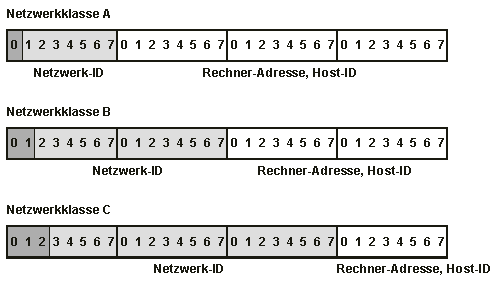
\includegraphics[scale=0.7]{Bilder/Netzwerkklassen.png}
			\end{center}
		
		\subsection{Subnetzmaske}
			Um ein bestehendes Computernetz zur besseren Übersicht und Verwaltung in mehrere kleine Netze aufteilen zu können, bedarf es einer Subnetzmaske. Diese gibt den Netzwerkbereich einer IP Adresse an. Mit Hilfe der Subnetzmaske kann außerdem überprüft werden, ob sich zwei Geräte im gleichen Subnetz befinden oder nicht. Verknüpft man IP Adresse und Subnetzmaske durch eine AND Verknüpfung, erhält man die Netzwerkkennung des Subnetzes, indem sich die IP Adresse befindet. Stimmen die Netzwerkkennungen zweier Systeme überein, befinden sie sich im selben Subnetz.
		
		\subsection{CIDAR}
			Die CIDAR ist eine vereinfachte Schreibweise für die Subnetzmaske. Da eine Subnetzmaske dadurch definiert wird, dass sie in binär Schreibweise eine fortlaufende Kette von gesetzten Bits haben muss, die nicht durch ein nicht gesetztes Bit unterbrochen werden darf, kann man die Schreibweise dahingehend vereinfachen, dass einfach die gesetzten Bits gezählt werden:
			\begin{center}
				\footnotesize
				\renewcommand{\arraystretch}{1.5}
				\begin{tabularx}{\columnwidth}{XXXXXXXXXXXXXXXXXXXXXXXXXXXXXXXX}
					1&2&3&4&5&6&7&8&9&10&11&12&13&14&15&16&\textcolor{red}{17}&18&19&20&21&22&23&24&25&26&27&28&29&30&31&32 \\
					\hline
					1&1&1&1&1&1&1&1&1&1&1&1&1&1&1&1&\textcolor{red}1&0&0&0&0&0&0&0&0&0&0&0&0&0&0&0 \\
				\end{tabularx}\\
				In diesem Falle wäre die CIDAR /17
			\end{center}
		
		\subsection{VLSM}
			VLSM ist ein erweitertes Subnetting. Hierzu wird die Subnetmaske in eine variable Länge gebracht um das Subnetz in mehrere verschieden große Teile zu unterteilen und sie hierarchisch nach ihrer Größe sortiert. Somit ist es möglich, Subnetze mit einer jeweils verschiedenen Anzahl an Hosts zu erschaffen, ohne dass dafür eine große Menge an IP-Adressen verschwendet werden muss.\vspace{.3cm}\newline
		\begin{minipage}[t]{.45\textwidth}
			Aufgabenstellung:
			\vspace{.2cm}\newline
			Es wird ein neues Gebäude gebaut. Dafür steht der IP-Bereich 11.137.4.0 /23 zur Verfügung. Die ersten 2 von den 6 Etagen sollen jeweils 100 IP-Adressen haben und die restlichen 4 jeweils 50 IP-Adressen. Gib die IP-Range jeder Etage an!
		\end{minipage}
		\hspace{1cm}
		\begin{minipage}[t]{.45\textwidth}
			Lösung:\vspace{.2cm}\newline
				\renewcommand{\arraystretch}{1.5}
				\begin{tabularx}{7.3cm}{|c|c|}
					\hline
					\cellcolor{cyan!60!white}Etage&\cellcolor{cyan!60!white}IP-Range \\
					\hline
					1&11.137.4.1   -  11.137.4.126 \\
					\hline
					2&11.137.4.129 -  11.137.4.254 \\
					\hline
					3&11.137.5.1   -  11.137.5.62 \\
					\hline
					4&11.137.5.65  -  11.137.5.126 \\
					\hline
					5&11.137.5.129 -  11.137.5.190 \\
					\hline
					6&11.137.5.193 -  11.137.5.254 \\
					\hline
				\end{tabularx}
		\end{minipage}
		
		\newpage
		
		\subsection{DMZ - Demilitarisierte Zone}
			Eine Demilitarisierte Zone bezeichnet ein Computernetz mit sicherheitstechnisch kontrollierten Zugriffsmöglichkeiten auf die daran angeschlossenen Server. Die in der DMZ aufgestellten Systeme werden durch eine oder mehrere Firewalls gegen andere Netze abgeschirmt.
			\begin{center}
				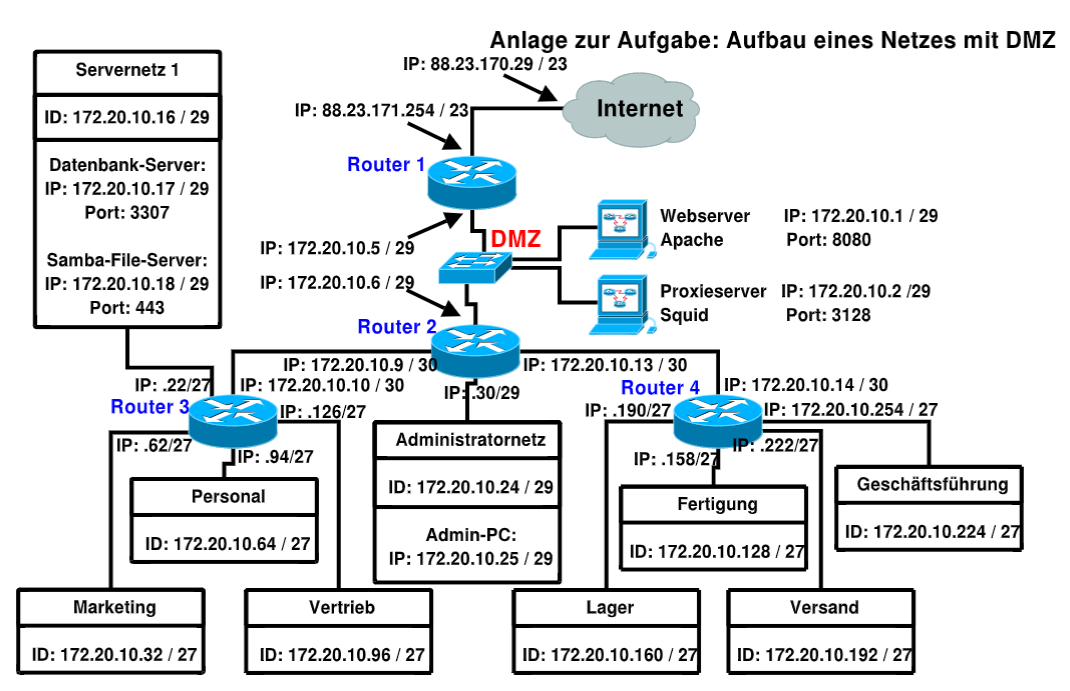
\includegraphics[scale=0.9]{Bilder/DMZ.PNG}
			\end{center}
		
		\subsection{IPv6 und IPv4 im Vergleich}
			Vorteile und Nachteile von IPv6 zu IPv4:
			\begin{table}[h]
				\renewcommand{\arraystretch}{1.5}
				\begin{tabularx}{17cm}{|X|X|}
					\hline
					\cellcolor{cyan!60}Vorteile&\cellcolor{cyan!60}Nachteile\\
					\hline
					\hline
					128 Bit = $\text{2}^{\text{128}}$ Adressen&Wenn jedes Gerät eine feste, statische Adresse bekommt, kommt es evtl. zu Sicherheitsrisiken \\
					\hline
					NAT wird nichtmehr gebraucht& \\
					\hline
					Broadcast-Adressen werden nichtmehr gebraucht& \\
					\hline
					ARP wird nichtmehr gebraucht& \\
					\hline
					bis zu 4GiB Datenversandt& \\
					\hline
					verbessertes Multicast& \\
					\hline
				\end{tabularx}
			\end{table}   
			
	\section{Codierung}
		\subsection{Huffmann-Codierung}
			Algorithmus zum \textbf{Komprimieren} von Dateien.\\
			\textbf{Idee:} Häufige Zeichen kurze Bit-Codierung, sodass Binär-Codierung möglichst kurz ist.
			\begin{enumerate}
				\item \textbf{Tabelle} mit vorkommenden Zeichen und deren Häuffigkeit erstellen
				\item \textbf{Binärbaum} mit Zeichen erstellen. Zeichen nach Häufigkeit sortiert. Zeichen mit geringster Häufigkeit zusammenfassen. Zusammengefasste zeichen weiter vereinen bis Baum vollständig ist
				\item \textbf{Codierung} der Zeichen aus Binärbaum lesen und in Tabelle schreiben
			\end{enumerate}
			\begin{center}
				\begin{figure}[!h]
					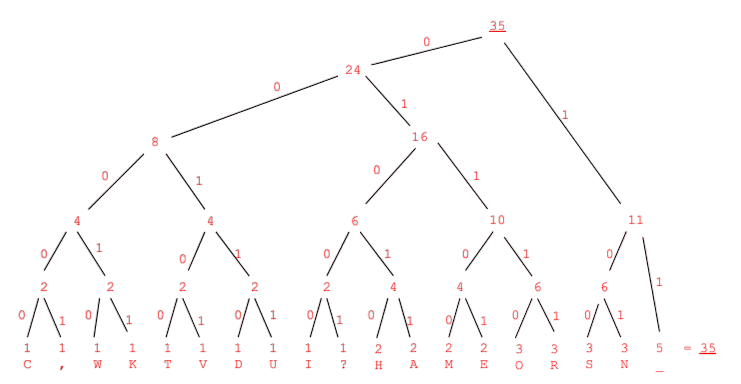
\includegraphics[width=\textwidth]{Bilder/Huffmann-Baum.png}
				\end{figure}
			\end{center}

		\subsection{Channel Coding}
			\begin{minipage}[c]{0.4\textwidth}
				\subsubsection{Fehlererkennung mit Paritätsbits}
				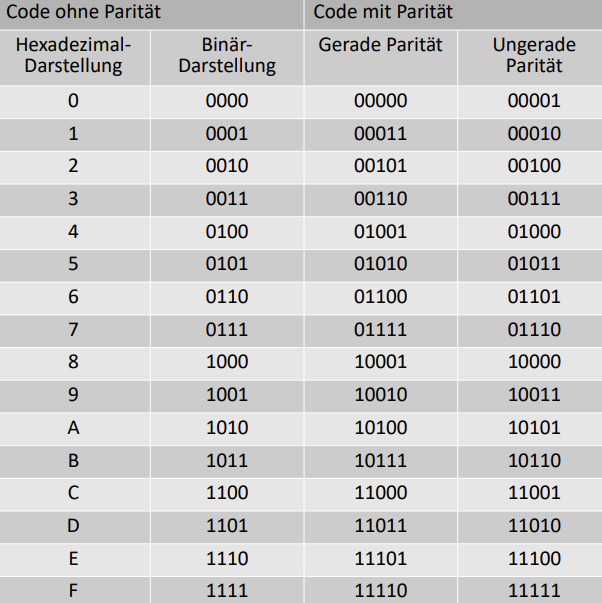
\includegraphics[width=\textwidth]{Bilder/paritaetsbit.png}
			\end{minipage}
			\begin{minipage}[c]{0.6\textwidth}
				\subsubsection{Fehlererkennung mit Hamming Distanz}
				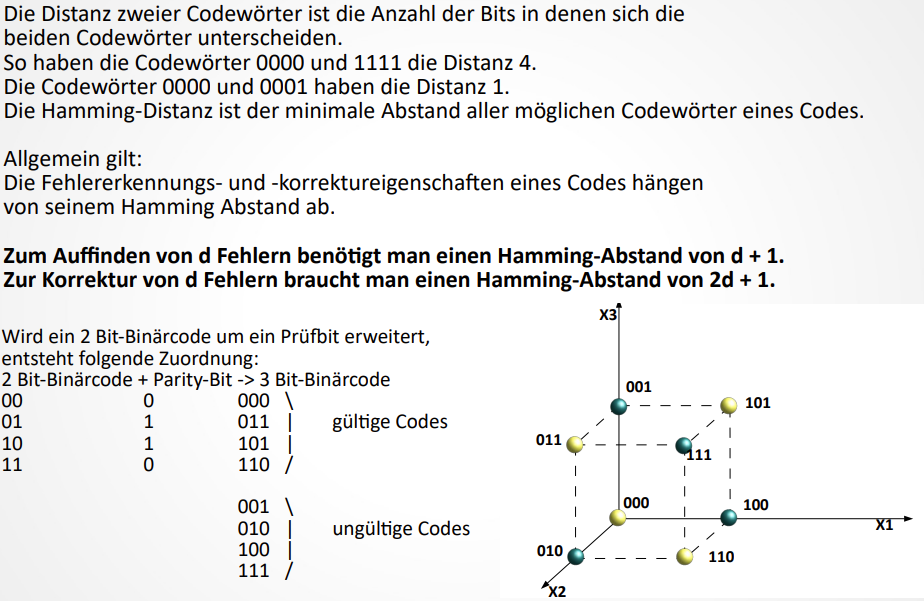
\includegraphics[width=\textwidth]{Bilder/hamming-distanz.PNG}
			\end{minipage}
			\subsubsection{Fehlererkennung mit 2-dimensionaler Parität}
				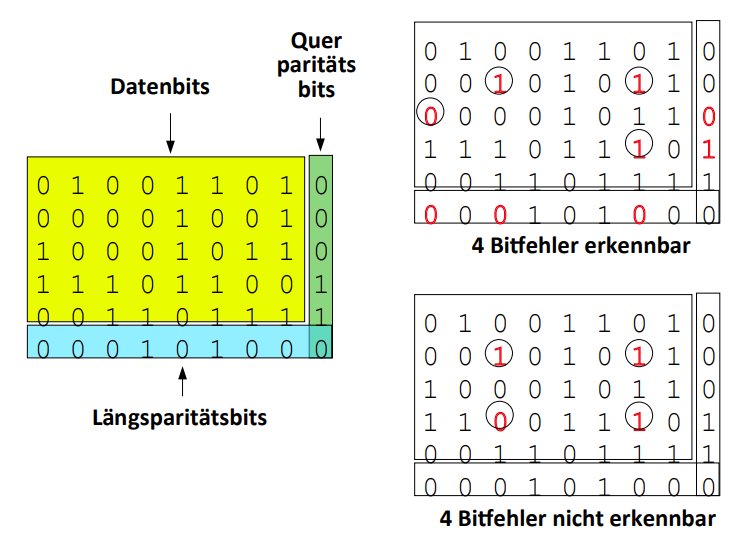
\includegraphics[width=\textwidth]{Bilder/2-dim-paritaet.PNG}
			\subsubsection{Fehlererkennung mit CRC(Cyclic Redundancy Check)}
				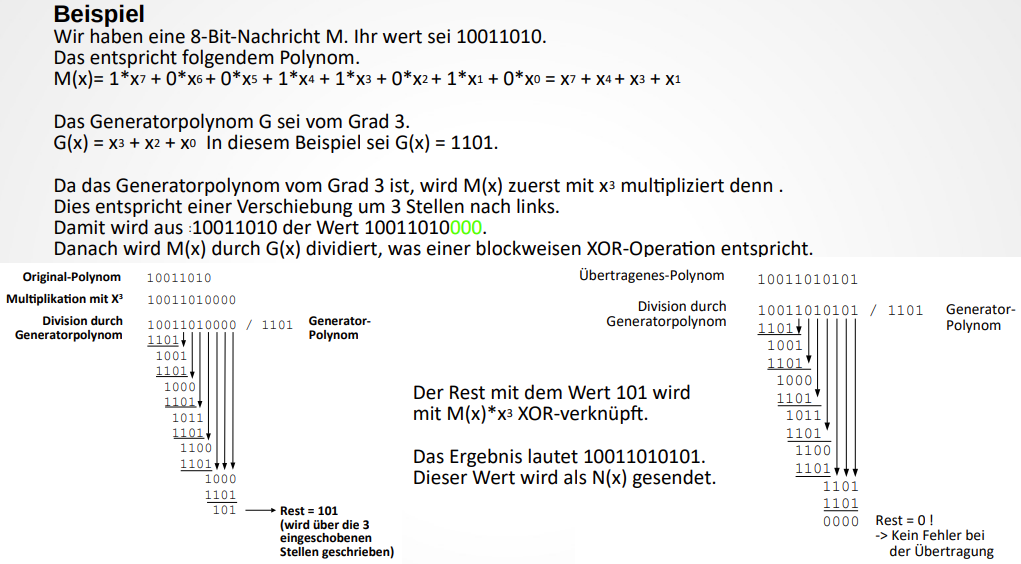
\includegraphics[width=\textwidth]{Bilder/crc1.PNG}
				Übliche CRC-Generatorpolynome sind:
				\begin{center}
					\begin{tabularx}{9cm}{X|l}
						\textbf{CRC}& \textbf{C(x) Generatorpolynom}\\
						\hline
						CRC-8& $X^8 + X^2 + X^1 + 1$\\
						CRC-10& $X^{10} + X^9 + X^5 + X^4 + X + 1$\\
						CRC-12& $X^{12} + X^{11} + X^3 + X^2 + 1$\\
						CRC-16& $X^{16} + X^{15} + X^2 + 1$\\
						CRC-CCITT& $X^{16} + X^{15} + X^5 + 1$\\
					\end{tabularx}
				\end{center}
			


\end{document}
